\section{Introduction}
\label{sec:intro}

A GNSS station velocity is a small number extracted from a long, noisy, interrupted
record. Its value is used in terrestrial reference frames \citep{altamimi2017pmm},
strain-rate fields \citep{kreemer2014gsrm} and loading studies
\citep{blewitt2002annual}, but its uncertainty is set less by the number of daily
solutions than by the time-correlated part of the coordinate error. A velocity
computed under a white-noise assumption can be optimistic by an order of
magnitude; the power-law noise model and the maximum-likelihood trajectory fit
that account for it are therefore not refinements but the basis of a defensible
velocity \citep{mao1999noise,williams2003coloured,amirisimkooei2007noise}.

Deep learning is now proposed for nearly every step before that fit: denoising,
gap filling and offset detection. Reported gains are large but rarely comparable,
because each study uses its own stations, its own metric and its own baseline.
The evaluation usually stops at signal recovery. A geodesist does not publish a
denoised series; they publish a velocity and an uncertainty, and a method can
improve recovery error while corrupting the noise estimate from which the
uncertainty is built.

This paper is a benchmark, not a new architecture. It asks a narrow question:
under one frozen protocol, on held-out real stations, does any learned method
beat a well-implemented classical one on the three tasks and on the products that
follow them? The answer is conditional rather than uniform. The parametric
baseline keeps its denoising advantage only while the truth stays inside its
basis; the learned gap filler wins at 30-day synthetic gaps once inference
matches training but does not beat linear interpolation on the full held-out
real set, and loses at long gaps; the learned detector orders large offsets
better but operates worse, and on real catalogue labels it trails in both $F_1$
and seed stability. The downstream product narrows the picture rather than
sharpening it: learned denoising reduces signal error, yet under the corrected
inference it neither improves nor degrades the velocity and its uncertainty.
The evidence behind this picture is stronger than in our first version in four
ways that matter.

First, the ground truth is no longer confined to the family the parametric
baseline assumes. In the earlier protocol the injected signal was a trend plus
constant harmonics, so the maximum-likelihood trajectory model was scored on its
own model family and removed about four-fifths of the injected error. We now
score the same methods on two truth families: an in-family signal built from a
real station's robust trajectory fit, and an out-of-family signal that adds
non-stationary seasonal amplitude, exponential transients and logarithmic
post-seismic relaxation. The parametric estimator loses its advantage when the
truth leaves its basis. The learned denoiser is nearly invariant across the two
families and, under protocol-matched inference, beats every model-free
decomposition in both; it remains far below the parametric estimator when the
truth sits in its basis.

Second, offset detection is evaluated against real catalogued offsets rather
than only against injected ones. We match the NGL discontinuity catalogue to the
held-out stations, keep labels inside each record and above the local noise
level, and score the classical detector and the learned detectors on the same
epochs. This removes the objection that synthetic offsets are easier than real
ones and tests the detectors where a geodesist would use them.

Third, training-seed variation is treated as part of the result. Denoising and
gap filling use ten seeds per architecture; detection uses twenty U-Net seeds
and ten TCN seeds. We report the
distribution over seeds, not a favourable draw, and we separate a fixed
read-out threshold from a threshold selected on held-out validation data. A
second architecture, a temporal convolutional network, is trained under the same
budget so that the conclusion is not a statement about one network.

Fourth, the downstream analysis includes a random-walk component. The first
version injected white plus flicker noise and left random walk open; here the
same velocity pipeline is run with and without a random-walk term, and the
effect on velocity bias, reported uncertainty and interval coverage is measured
rather than assumed. The benchmark also carries a second analysis centre: the
NGL long records are the primary set, and the held-out JPL series form an
external validation arm. JPL series from training sites contribute to training,
but no held-out site, from either centre, is ever seen by a learned method
before scoring.

The contributions are:

\begin{enumerate}
\item A reproducible benchmark of 333 daily series from 321 sites, with a
station-level 60/20/20 split (198/68/67 series, 193/64/64 sites), frozen station
lists, fixed seeds and released result files (Sec.~\ref{sec:data}).
\item A two-family ground-truth protocol that separates in-family from
out-of-family truth and shows how much of the classical advantage in the
earlier benchmark came from the truth sitting inside the parametric basis
(Sec.~\ref{sec:results:t1}).
\item A real-label offset study on 153 held-out component series from 58
stations, using 1\,743 catalogued discontinuities, with amplitude- and
signal-to-noise-stratified scores and detection delays
(Sec.~\ref{sec:results:t3:real}).
\item Seed- and architecture-robust comparisons for denoising, gap filling and
detection, including parameter counts, training cost and validation-based
threshold selection (Secs.~\ref{sec:results:t1}--\ref{sec:results:t3}).
\item A downstream propagation study under white-plus-flicker and
white-plus-flicker-plus-random-walk noise, reporting velocity bias, uncertainty
calibration and coverage, plus an external JPL arm and a regional holdout
(Secs.~\ref{sec:results:downstream} and~\ref{sec:results:external}).
\end{enumerate}

Section~\ref{sec:related} positions the benchmark against the four literatures it
joins. Section~\ref{sec:data} describes the data and the split,
Sec.~\ref{sec:method} the protocol and methods, and Sec.~\ref{sec:results} the
results. Section~\ref{sec:discussion} states the boundary of the conclusion and
its limitations, and Sec.~\ref{sec:conclusion} answers the question posed above.

\begin{figure}[t]
\centering
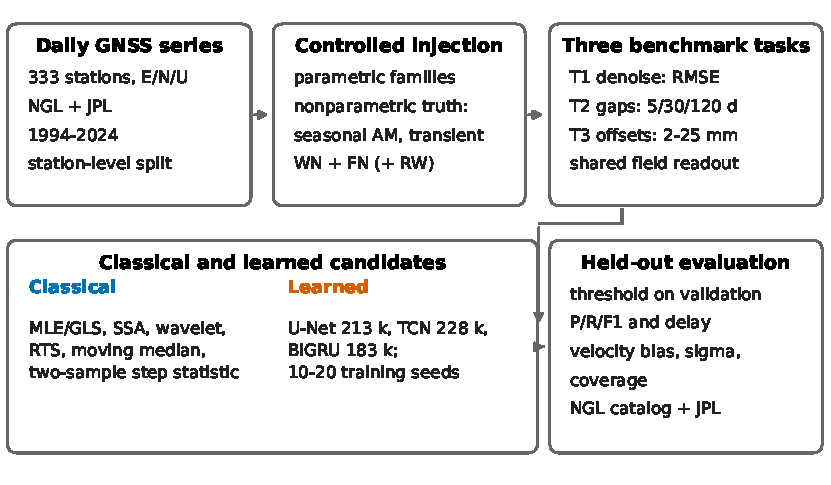
\includegraphics[width=\linewidth]{figures/fig01_pipeline.pdf}
\caption{The benchmark pipeline. Real daily series are injected with a known
signal and noise model, the resulting realisation is scored on the three tasks
by classical and learned candidates under one read-out rule, and each output is
carried into the velocity and noise estimation. The downstream step is what
separates a processing benchmark from a signal-recovery benchmark.}
\label{fig:pipeline}
\end{figure}
